\documentclass[12pt]{article}

\pagestyle{empty}
\setcounter{secnumdepth}{2}
%----------------------------------------------------------------------------------------
%   Packages and configurations
%----------------------------------------------------------------------------------------
\usepackage[dutch]{babel}
\usepackage{hyperref} %Allow for references
\hypersetup{
    colorlinks,
    citecolor=black,
    filecolor=black,
    linkcolor=black,
    urlcolor=black
} %Set up hyperlink colours.
\newcommand{\sectionbreak}{\clearpage} % Should start every section on its own page
\usepackage{geometry} % Required to change the page size to A4
\geometry{a4paper} % Set the page size to be A4 as opposed to the default US Letter
\usepackage{chngpage}
\usepackage{appendix}
%REMOVE IF HEADER/FOOTER BROKEN
\usepackage{fancyhdr} % Required for custom headers
\usepackage{extramarks} % Required for headers and footers
\usepackage{lastpage} % Required to determine the last page for the footer
%-----------------1
\topmargin=0cm
\oddsidemargin=0cm
\textheight=22.0cm
\textwidth=16cm
\parindent=0cm
\parskip=0.15cm
\topskip=0truecm
\raggedbottom
\abovedisplayskip=3mm
\belowdisplayskip=3mm
\abovedisplayshortskip=0mm
\belowdisplayshortskip=2mm
\normalbaselineskip=12pt
\normalbaselines
\usepackage{listings}
\usepackage[svgnames,table,xcdraw]{xcolor}
\lstset { 
    language=C,
    frame=single,
    escapeinside={\%*}{*)}, 
    breaklines=true,  
    backgroundcolor=\color{black!5},
    basicstyle=\footnotesize,
    commentstyle=\color{mygreen},
    numberstyle=\tiny\color{mygray},
    rulecolor=\color{black},
    keywordstyle=\color{blue},
}
\definecolor{mygreen}{rgb}{0,0.6,0}
\definecolor{mygray}{rgb}{0.5,0.5,0.5}
\definecolor{mymauve}{rgb}{0.58,0,0.82}
\usepackage{wasysym}
\pagestyle{fancy}
\lhead{\textsc{Beckett,} \textsc{Braat} \& \textsc{Mathijssen}} % Top left header
\rhead{Opdrachten week 4} % Top center header
\lfoot{
\includegraphics[height=0.8cm]{avans}} % Bottom left footer
\cfoot{} % Bottom center footer
\rfoot{Pagina\ \thepage} % Bottom right footer
\renewcommand\headrulewidth{0.4pt} % Size of the header rule
\renewcommand\footrulewidth{0.4pt} % Size of the footer rule
\usepackage{graphicx} % Required for including pictures

\usepackage{float} % Allows putting an [H] in \begin{figure} to specify the exact location of the figure
\usepackage{wrapfig} % Allows in-line images such as the example fish picture
\usepackage{lipsum} % Used for inserting dummy 'Lorem ipsum' text into the template
\usepackage{pdfpages}
\usepackage[font={footnotesize}]{caption}
\graphicspath{ {../Images/Logos/}{../Images/}{../Images/Week1/} {../Images/Week2/}{../Images/Week3/}{../Images/Week4/}}
\setlength\parindent{0pt} % Removes all indentation from paragraphs
%\usepackage{showframe}
\newcommand*{\SignatureAndDate}[1]{%
    \par\noindent\makebox[2.5in]{\hrulefill} \hfill\makebox[2.0in]{\hrulefill}%
    \par\noindent\makebox[2.5in][l]{#1}      \hfill\makebox[2.0in][l]{Date}%
}%Signature package
\begin{document}
\begin{titlepage}
\pagenumbering{Roman}
\newcommand{\HRule}{\rule{\linewidth}{0.5mm}} % Defines a new command for the horizontal lines, change thickness here

\center % Center everything on the page


\includegraphics[height=3cm] {avans}\\% Include a department/university logo - this will require the graphicx package
\textsc{\Large Avans Hogeschool Breda}\\[0.5cm] % Major heading such as course name
\textsc{\large Intelligente wireless sensornetwerken }\\[0.5cm] % Minor heading such as course title
\HRule \\[0.4cm]
{ \huge \bfseries Opdrachten week 3	}\\[0.4cm] % Title of your document
\HRule \\[1.5cm]

\begin{minipage}{0.4\textwidth}
\begin{flushleft} \large
\emph{Auteurs:}\\
Guus \textsc{Beckett} \\% Your name 
Joris \textsc{Mathijssen}\\
Jelle \textsc{Braat} % Your name 
\end{flushleft}
\end{minipage}
~
\begin{minipage}{0.4\textwidth}
\begin{flushright} \large
\emph{Docenten:} \\
Diederich \textsc{Kroeske} \\ % Supervisor's Name
Andries \textsc{van Dongen} \\ % Supervisor's Name
\end{flushright}
\end{minipage}\\[4cm]

{\large \today}\\[3cm] % Date, change the \today to a set date if you want to be precise

Versie: 0.2.0

\vfill % Fill the rest of the page with whitespace

\end{titlepage}

\clearpage
% \section*{Voorwoord}
% \addcontentsline{toc}{section}{Voorwoord}

% Guus Beckett \& Jim van Abkoude \\
% \today \\
% Breda
% \newpage
% \section*{Samenvatting}
% \addcontentsline{toc}{section}{Samenvatting}
% \lipsum[0-2]
% \newpage
% \tableofcontents
% \newpage
\pagenumbering{arabic}
\section*{Opdracht 1 a}
\begin{quote}
Gebruik het programma X-CTU voor de configuratie van de nodes: \\
- coördinator api, met een zelfgekozen PANID, broadcast destination adres en identificatienaam(NI) \\
- router api, (2x) met het gekozen PANID, destination adres 0x00 (= de coördinator) en een eigen identificatienaam,\\
- end-device met het gekozen PANID, destination adres 0x00 (= de coördinator) en een eigen identificatienaam.
\end{quote}
We hebben de xbees geprogrammeerd volgends de opgegeven voorwaarden. Alle 4 hebben de correcte instellingen zoals je kan zien in deze afbeelding.
\begin{figure}[H]
\captionsetup{justification=raggedright,
singlelinecheck=false
}
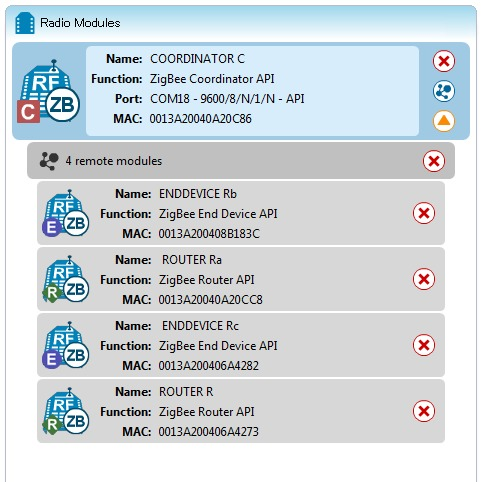
\includegraphics[scale=0.8] {1a-een}
\caption{Lijst van gekoppelde devices.}
\end{figure}
\clearpage
\begin{figure}[H]
\captionsetup{justification=raggedright,
singlelinecheck=false
}
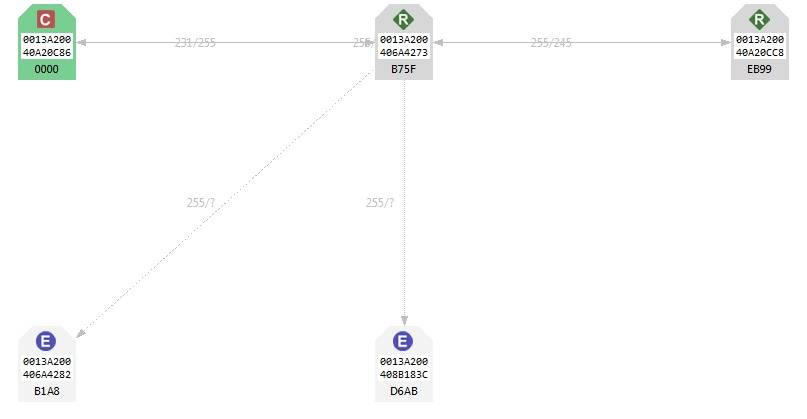
\includegraphics[scale=0.8] {1a-drie}
\caption{Overzicht van de verbindingen tussen de devices}
\end{figure}
\begin{figure}[H]
\captionsetup{justification=raggedright,
singlelinecheck=false
}
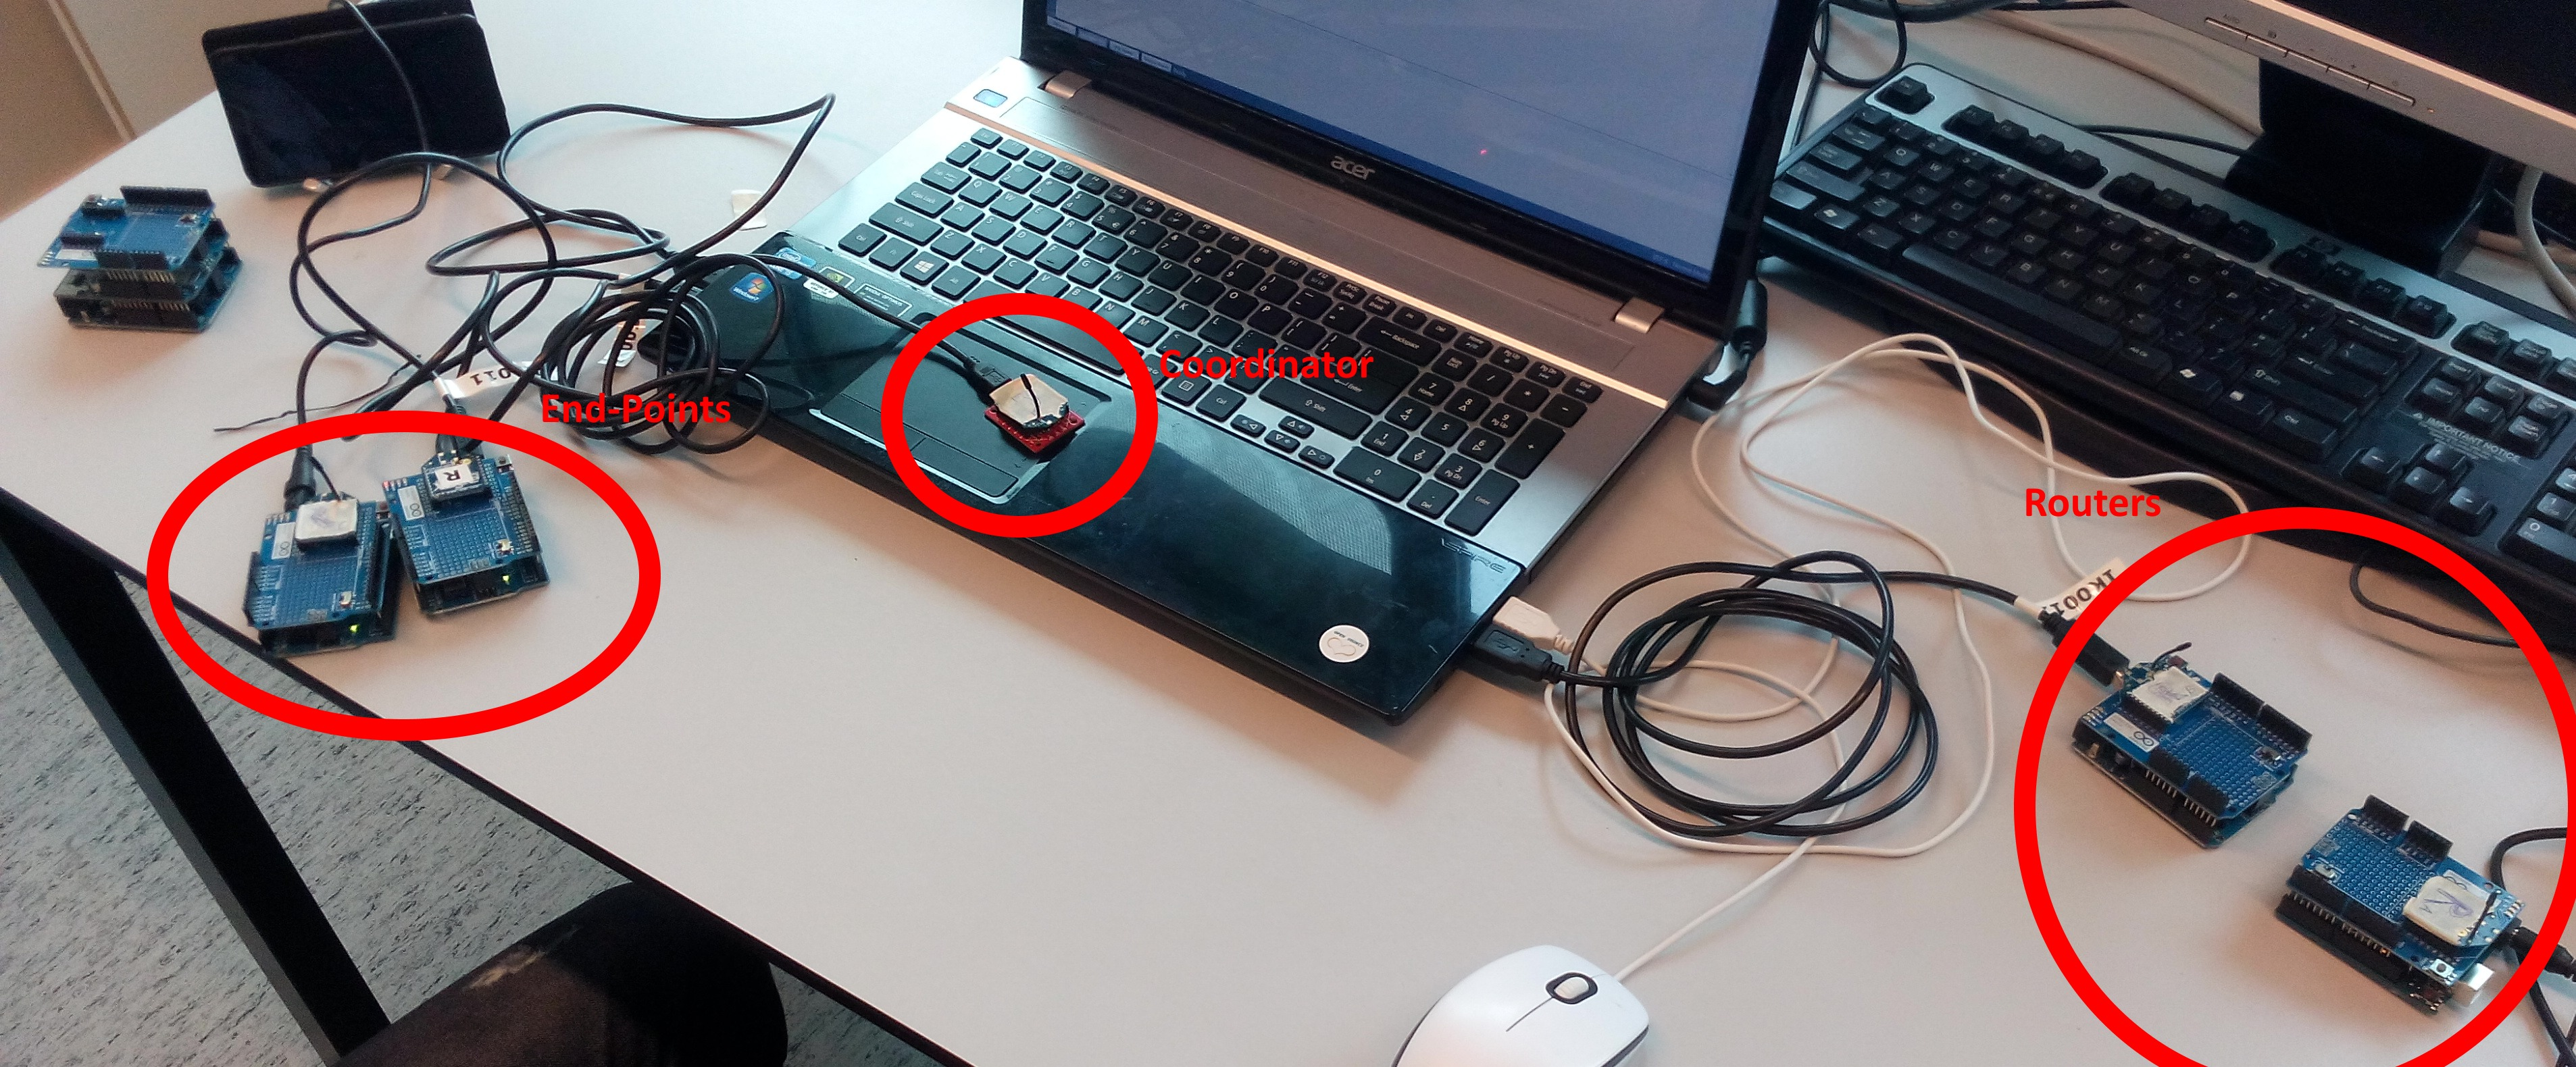
\includegraphics[scale=0.1] {1a-twee}
\caption{Setup van de devices op tafel}
\end{figure}
\newpage
\section*{Opdracht 1 b}
\begin{quote}
Sluit vervolgens de coordinator aan op de PC met ZigBee Operator, en sluit de andere nodes 	aan 	op een Arduino met XBee shield of ook via een USB-Explorer. Tekst de werking van de configuratie met het programma ‘ZigBee Operator’. Bekijk de configuratie. Noteer de 64-bits en 16-bits netwerk adressen van de nodes.
\end{quote}
\begin{table}[h]
\begin{tabular}{|l|l|l|l|l}
\cline{1-4}
 Operator & 64bit address High & 64bit address Low & 16bit address &  \\ \cline{1-4}
 Coordinator & 0013A200 & 40A20C86  & 0000 \\ \cline{1-4}
 Router A & 0013A200 & 406A4273 & B75F &  \\ \cline{1-4}
 Router B & 0013A200 & 40A20CC8 & EB99 &  \\ \cline{1-4}
 Endpoint A & 0013A200 & 408B183C & D6AB &  \\ \cline{1-4}
 Endpoint B & 0013A200 & 406A4282 & B1A8 &  \\ \cline{1-4}
\end{tabular}
\end{table}
\newpage
\section*{Opdracht 1 c}
\begin{quote}
Configureer de end-devices via USB-Explorer of via ‘Remote AT Command’ voor het genereren van periodieke IO datasamples (in dit voorbeeld elke 60 s). Commands DO,D1 en IR, SM=4, SP = 0x3E8 (10s), SN=6, SO=0, ST=0x1F4 (500 ms wakker)).

	Controleer e.e.a. met ‘ZigBee Operator’
\end{quote}
\begin{figure}[H]
\captionsetup{justification=raggedright,
singlelinecheck=false
}
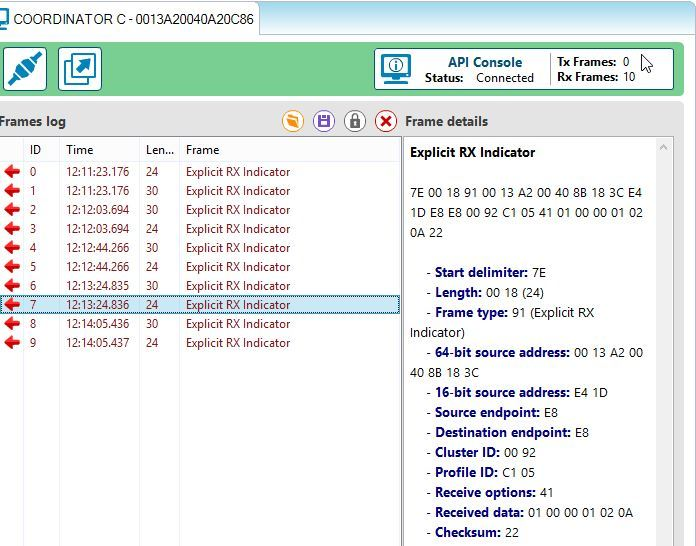
\includegraphics[scale=0.7] {1c-een}
\caption{terug gave van de data API console}
\end{figure}
\newpage
\section*{Opdracht 1 d}
\begin{quote}
	Je kunt de sensornode (end-device met sensor) zo inrichten dat de sensor (of sensoren)\\ a) aangesloten is op de XBee-node zodat deze zelf de sensor data verwerkt, of dat \\ b) de sensor aangesloten is op de Arduino en op de Arduino een programma draait dat de 	sensoren uitleest en deze toestuurt aan de bijbehorende XBee-module. Realiseer een van beide opties voor de temperatuursensor  \\
- Schrijf een programma voor (Arduino van) de coördinator-node dat zorgt voor de verwerking van de binnenkomende data. \\
- Stuur deze data naar een feed op COSM (zoals in week 3)
\end{quote}

\begin{figure}[H]
\captionsetup{justification=raggedright,
singlelinecheck=false
}
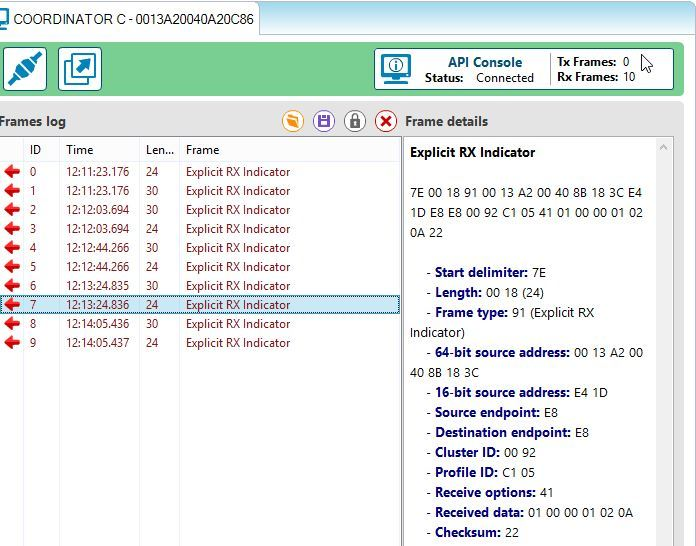
\includegraphics[scale=0.7] {1c-een}
\caption{terug gave van de data API console}
\end{figure}
\begin{lstlisting}
\end{lstlisting}
\end{document}
